\documentclass{article}
\usepackage{fullpage}
\usepackage[pdftex]{graphicx}
\usepackage{hyperref}
\usepackage[usenames,dvipsnames]{color}
\usepackage{amssymb}
\usepackage{amsmath,amsfonts}
\usepackage{comment}
\usepackage[utf8]{inputenc}
\usepackage[T1]{fontenc}
\usepackage{listings}
\usepackage[finnish]{babel}
\usepackage{float}
\usepackage{moreverb}
\usepackage[titletoc]{appendix}
\usepackage[nottoc]{tocbibind}
\usepackage{afterpage}
\usepackage{multirow}
\usepackage{longtable}
% settings
\addtolength{\parskip}{\baselineskip}
\setlength\parindent{0pt}	% remove indent
\afterpage{\clearpage}
\let\oldsection\section
%\renewcommand{\section}{\clearpage\oldsection} % pagebreak before every new section

% kuvaa{suhteellinen leveys}{tiedosto}{kuvateksti}{label}
% kuva{nimi} täydellä leveydellä
\newcommand{\kuvaa}[4]{%
	\begin{figure}[h]%
		\centering \includegraphics[width=#1\textwidth]{#2}%
		\caption{#3 \label{fig:#4}}%
	\end{figure}%
}
\newcommand{\kuva}[2]{\kuvaa{0.99}{#1}{#2}{#1}}

% taulukoiden defaultit on ihan jäätävän tiiviitä
\setlength{\tabcolsep}{4pt}
\renewcommand{\arraystretch}{1.2}

\begin{document}

% coverpage erikseen eka, jätetään titlesivu myös wikiversioon
%\begin{titlepage}
\begin{center}

\textsc{ \LARGE Loppuraportti:AS-0.3200 Automaatio- ja systeemitekniikan projektityöt }\\[1.5cm]

\textsc{ \Large A13-10 Radio-ohjattavan pienoismallin ohjausjärjestelmän ja käyttöliittymän kehittäminen }\\[0.5cm]

\begin{tabular}{ l | p{12cm} }
	\hline
	Aloituspäivämäärä & 17.9.2013\\

	\hline
	Lopetuspäivämäärä & 15.12.2013\\

	\hline
	\multirow{3}{*}{Tekijät}
	& Lasse Kortetjärvi, 230579, AUT. lasse.kortetjarvi@aalto.fi\\
	& Toni Liski, 81911C, AUT. toni.liski@aalto.fi\\
	& Konsta Hölttä, 79149S, AUT. konsta.holtta@aalto.fi\\

	\hline
	Valvoja & Arto Niskanen\\

	\hline
	\multirow{8}{*}{Työohje} &
	\begin{itemize}
	\item Ohjausjärjestelmä: ABS- ja ESC-toiminnot sisältävän ohjausjärjestelmän jatkokehitys\begin{itemize}
	\item Mikrokontrollerikoodin ominaisuuksien kehittäminen
	\item Ajonvakautusalgoritmien toteutuksen parantelu
	\end{itemize}

	\item Käyttöliittymä: Matlab-pohjaisen käyttöliittymän jatkokehitys \begin{itemize}
	\item Ennalta suunniteltujen ajosyklien ja ajotilanteiden suorittaminen
	\item Ajotietojen tallentaminen ja analysointi
	\end{itemize}
	\item Kauko-ohjaus: Manuaalisen kauko-ohjauksen toteutus.
	\end{itemize} \\

	\hline
	\multirow{3}{*}{Opintopisteet}
	& Lasse Kortetjärvi: 4 \\
	& Toni Liski: 4 \\
	& Konsta Hölttä: 5 \\

	\hline
\end{tabular}

\vfill

{\large \today}

\end{center}
\end{titlepage}


% normaali titlesivu kuolevaisille
\title{
Radio-ohjattavan pienoismallin ohjausjärjestelmän ja käyttöliittymän kehittäminen \\
Loppuraportti \\
~\\
AS-0.3200 Automaatio- ja systeemitekniikan projektityöt, ryhmä~A13-10
}

\author{Toni Liski, Konsta Hölttä, Lasse Kortetjärvi}
\date{15.12.2013}

% Title page
\maketitle
\thispagestyle{empty}
\clearpage

\tableofcontents
\clearpage

\section{Projektin tavoite}

\subsection{Tausta}
Projektin taustana on Aalto-yliopiston Insinööritieteiden korkeakoulun Koneenrakennustekniikan kurssi Kon-16.4081 Ajoneuvojen tuotekehitys. Kurssilla aloitettiin vuonna 2011 projekti, jonka tarkoituksena oli rakentaa radio-ohjattavan auton pienoismalli ajodynamiikan opetuskäyttöön. Syksyllä 2012 Automaatio- ja systeemitekniikan projektityökurssilla autoon tehtiin osaprojektina Matlab-käyttöliittymä ja rakennettiin ohjelmisto ABS- ja ESP-ohjauksille, ja samalla samana vuonna ajoneuvokurssilla kehitettiin auton mekatroniikkaa yleisellä tasolla. Molemmat projektit jäivät kuitenkin kesken, ja tänä vuonna niitä jatkettiin kummankin laitoksen osalta. Kon-16.4081-kurssin projektiryhmässä työskenteli vuoden ajan viisi henkilöä ja Automaatio- ja systeemitekniikan projektityökurssilla syksyn ajan kolme henkilöä. Kuvassa \ref{fig:ryhmajako} alkuperäinen suunnitelma ryhmäjaoksi.

\kuvaa{0.8}{ryhmajako}{Alkuperäinen ryhmäjakosuunnitelma.}{ryhmajako}

\subsection{Tehtävä}
Projektin tehtävänä oli kehittää yllämainittuun kauko-ohjattavaan autoon toimivat lukkiutumattomien jarrujen (ABS) ja ajoneuvonhallintajärjestelmän (ESP) ohjaukset, kehittää auton käyttöliittymää ja toteuttaa automaattiohjaus etukäteen määriteltyjen reittipisteiden avulla. Lisäksi autoon oli tarkoitus lisätä etäisyysanturit helpottamaan paikoitusta testialustalla, eli tässä tapauksessa juoksumatolla. Samoja antureita oli tarkoitus hyödyntää myös ennaltaehkäisemään ajoneuvon törmäyksiä kiinteisiin kohteisiin. Lopuksi, jos projektissa jäisi aikaa, olisi tarkoituksena toteuttaa kauko-ohjaus esimerkiksi RC-auton kauko-ohjainta käyttäen, sekä käyttää etäisyysantureita automatisoimaan kulku seinää tai monimutkaista rataa vasten.

\subsection{Rajaus}
Projekti rajattiin ohjaus- ja säätöjärjestelmien kehitykseen, käyttöliittymäkoodin parantamiseen ja muutamien testausta helpottavien antureiden lisäämiseen. Pyrimme minimaalisiin muutoksiin valmiissa komponenteissa ja elektroniikassa.

\subsection{Tavoite}
Tavoitteena oli projektin lopuksi päästä testaamaan autoa eri ympäristöissä siten, että auton ohjelmisto ja säätöjärjestelmät olisivat täysin kunnossa ja helposti jatkokehitettävissä. Tavoitteena oli myös auton helppo kauko-ohjaus joko Matlab-käyttöliittymän kautta näppäimistön avulla, tai erillisellä kauko-ohjaimella tai joystickillä.

\section{Lähtötilanne}
Kuten projektit yleensä, tämäkään ei mennyt - tai edes lähtenyt käyntiin - aivan niin kuin suunniteltiin. Hyvin pian projektin alussa huomasimme, että auton tilasta saadut lähtötiedot olivat vakavasti puutteellisia ja osittain jopa vääriä. Auto ei todellakaan ollut siinä tilassa, että ABS:ää olisi voinut testata tai käyttöliittymää olisi kannattanut lähteä laajentamaan nykyisestä tilastaan. Auto ei itseasiassa edes liikkunut, sillä siinä oli väärin mitoitettuna niin akut, moottorit, nopeudensäätimet kuin voimansiirtokin - jarruservoista puhumattakaan.

Auton ohjelmistotkin oli kasattu monen projektin aikana pienistä palasista, eikä kokonaisuutta oltu koskaan oikein mietitty. Sen näki muun muassa siitä, että kaikki koodi - sekä käyttöliittymässä että mikrokontrollereissa - oli kirjoitettu yhteen tiedostoon prototyypinomaisesti ``tällä se nyt toimi'' -tyylillä, ilman minkäänlaista modulaarisuutta. Ohjelmistojen jatkokehittäminen tästä tilasta olisi ollut vähintään tyhmää ja tuskallista, eikä ainakaan reilua käyttäjille tulevaisuudessa.

Projektin alkuvaihe menikin, suunnitelmista poiketen, pitkälti auton nykytilan selvittämiseen ja mahdollisten korjausten suunnitteluun. Huomattiin nopeasti, että projekti ei tule valmistumaan suunnitelmien mukaisesti ajallaan, eikä kaikkia suunniteltuja ominaisuuksia pystytä mitenkään toteuttamaan. Lisäksi Ajoneuvon tuotekehityskurssin ryhmän palaveriin osallistuttuamme meille selvisi, että heillä on tavoitteena saada auto ajokuntoon juuri ennen joulua, joten mekään emme pääsisi ajamaan autolla ennen sitä. Jouduimme siis muuttamaan suunnitelmia radikaalisesti ja keskittymään lähinnä auton simulointiin ja jo olemassaolevien ominaisuuksien korjaamiseen ja parantamiseen. Yksi tällaisista ominaisuuksista oli valmiina oleva protokolla ja sen koodi, jotka katsottiin joustamattomuutensa vuoksi hankalaksi jatkokehittää.

Alkuperäinen syy, minkä vuoksi tämä projekti AS-projektikurssille tuli, oli epäillys ABS-jarrujen toimimattomuudesta. Tehtävänantona olikin ABSien ja ESP:n korjaaminen ja jatkokehittäminen. Epäilys algoritmien toimimattomuudesta osottautui kuitenkin vääräksi, mutta mekaaniset rajoitteet tekivät suunnitellun säätimen käytöstä mahdotonta.

Projektin edetessä tuimme osaamisellamme toista ryhmää ja yhteistuumin päätimme tilata ajoneuvoon uudet moottorit, nopeudensäätimet ja akut. Lisäksi autoon tilattiin etäisyysanturit sivuille ja eteen. Uudet akut tulivatkin riittävän ajoissa siten, että saimme loppudemossa ajettua autolla muutamia metrejä käyttäen kuitenkin vanhaa voimansiirtoa, moottoreita ja nopeudensäätimiä. Toisen renkaan voimansiirtoon käytetty kulmavaihde oli jo kulunut loppuun väärän mitoituksen vuoksi, mutta toisella renkaalla ajaminen onnistui kaikkien suureksi yllätykseksi kohtuullisen hyvin (metelistä ja valtavasta virrankulutuksesta huolimatta). Vaikka kytkin vielä säätöjenkin jälkeen luisti, kului toisenkin renkaan kulmavaihde pian olemattomaksi.

Tarkempi kuvaus auton alkutilasta löytyy syksyn 2012 projektiryhmän loppuraportista~\cite{bib:loppuraportti}, sekä vuoden 2012 Ajoneuvon tuotekehitys -kurssin loppuraportin liitteestä 5 (mekatroniikka)~\cite{bib:mekatroniikka}.

\section{Rakenne ja osa-alueet}
\subsection{Jarrut}
Jarrujärjestelmä on toteutettu FG Modellsportin vaijerikäyttöisillä levyjarruilla joita säädetään pienoismalleista tutuilla analogisilla RC-auton servoilla ja omituisen löysillä palautusjousilla. Tällainen vaijerikäyttöinen mekanismi on hyvin altis välyksille, kitkalle sekä venymiselle, mistä muodostuu säätöpiiriin viiveitä ja epälineaarisuuksia. Tällaiselle systeemille on mitattu 2,5 Hz:n taajuusvaste, kun sen tulisi olla yli 100 Hz jotta ABS-säätö olisi mahdollinen \cite{bib:testbed}.
RC-auton servo on paikkaohjattu aktuaattori, jota ohjataan 50 Hz:n PWM-signaalilla. Paikkaohjaus tuo haasteita järjestelmässä missä ohjattavana suureena on jarruvoima. Tämä tarkoittaa sitä, että säätöjärjestelmä on erittäin herkkä muutoksille, ja jos järjestelmässä tulee esimerkiksi välystä niin samaan paikkaan ohjattu servo ei enää tuotakaan samaa voimaa. Tämän korjaamiseksi suunniteltiin servoihin uudet piirilevyt, joista on poistettu takaisinkytkentä ja servot toimivat normaaleina DC-moottoreina. Näin voidaan ohjata suoraan servomoottorin tuottamaa voimaa. Uusissa ohjaimissa käytettiin Vishayn Si9986 \cite{bib:hbridge} H-siltaa, jolla voidaan ohjata moottorin kierroslukua ja pyörimissuuntaa PWM-signaalilla.
Uudet piirilevyt ovat valmistusteknisistä seikoista johtuen vielä tällä hetkellä työn alla.

\subsection{ABS-järjestelmä}
ABS- ja ESP-järjestelmien algoritmien laskutoimitusten epäiltiin olevan hitaita niissä käytettyjen laskutoimitusten vuoksi. Tätä tutkittiin lisäämällä algoritmien suoritusten väliin suoritusaikaa mittaavia laskureita. Kuvassa \ref{fig:exectimes} on esitetty mikrokontrollereiden eri syklien kumulatiivisten suoritusaikojen vaihtelu. Huomataan, että molemmat kontrollerit suoriutuvat hyvin tehtävistään säädetyssä 10 ms:n suoritussyklissä. Yhtään ylivuotoakaan ei testiajon aikana ilmennyt, eli kaikki tehtävät tulivat jokaisella syklillä suoritettua.

\kuvaa{0.8}{exectimes}{Alkuperäisten mikrokontrollerien syklien suoritusajat}{exectimes}

Koska alunperin määriteltyä ABS-järjestelmän jatkokehittämistä ei päästy RC-auton testaamisen muodossa tekemään, simuloitiin mahdollisia vaihtoehtoisia säätöjärjestelmiä. 

Ajoneuvon hidastuvuus määräytyy renkaan jarrutusvoiman

\begin{equation} \label{eq:fr}
	F_r = \mu G_p
\end{equation}

mukaan, missä $F_r$ on jarrutusvoima, $\mu$ on tien ja renkaan välinen kitkakerroin ja $G_p$ on renkaalla oleva paino. Simulaatioissa käytettiin neljännesajoneuvon massaa $9/4$ kg. Käytettävissä oleva kitkakerroin tietyllä alustalla riippuu renkaan luistosta\cite{bib:milliken} ja optimoimalla luisto saavutetaan paras hidastuvuus. Esimerkki renkaan jarrutusvoiman tuotosta luiston funktiona on esitetty kuvassa \ref{fig:slip}.

\kuvaa{0.8}{frVsSlip}{Renkaan jarrutusvoiman tuotto luiston funktiona \cite{bib:milliken}.}{slip}

Alkuperäinen ohjelmistokoodi perustui menetelmään, jossa renkaiden kiihtyvyyksien mukaan säädetään jarrutusvoimaa \cite{bib:bosch}. Tämä oli toteutettu siten, että parametrein säädettävien rajakiihtyvyyksien mukaan vaihdeltiin tilaa eri jarrutusvaiheiden välillä. Tätä pyrittiin uudessa järjestelmässä parantamaan huomioimalla säädössä renkaan kiihtyvyyden lisäksi myös renkaan luisto. Tämä on määritetty seuraavan kaavan mukaan:

\begin{equation}
	S = 1 - \frac{\omega_w}{\omega_v}
\end{equation}

missä $S$ on luisto, $\omega_w$ on renkaan kulmanopeus ja $\omega_v$ on ajoneuvon kulmanopeus. Jos luisto $S$ on $0$, renkaan ja ajoneuvon kulmanopeuksissa ei ole eroa, ja jos luisto $S$ on $1$, niin rengas on täysin lukittunut.

Renkaan luisto jarrutuksen aikana otettiin huomioon uuden säätimen suunnittelussa, ja näin pyrittiin optimoimaan ajoneuvon hidastuvuutta. Säätimen periaatekaavio on esitetty kuvassa \ref{fig:absmdl}. Etukäteen määritellyn rengasmallin mukaan määritellään optimaalinen luisto, jonka perusteella pyritään säätämään jarrutusvoimaa. Jos kuitenkin renkaan kiihtyvyys/hidastuvuus kasvaa yli säädettyjen maksimi- ja minimiarvojen, alkaa se muuttaa painotuskerrointa K, jolloin kiihtyvyyssäädin saa suuremman painoarvon. Tällöin pyritään äkilliset muutokset korjaamaan kiihtyvyyssäätimellä ja hienosäätämään jarrutustapahtumaa luiston perusteella.

\kuvaa{0.8}{mdl}{ABS-säätimen lohkokaavio.}{absmdl}

Simulaatiomallissa jarrujärjestelmää kuvattiin mallilla

\begin{equation}
	J_w \dot \omega = F_r R_w - \tau_\text{brake}
\end{equation}

jossa $J_w = 9*10^{-4} \text{kg} \text{m}^2$, $F_r$ kaavasta \ref{eq:fr}, $R_w = 0.0625 \text{m}$, sekä jarruttava momentti $\tau_\text{brake} = \text{brakepos} * 1.408*10^{-4} Nm$. Jarruttavan momentin kerroin on arvioitu olemassa olevasta jarrujärjestelmästä. Lisäksi mallissa otettiin huomioon viive, joka on olemassa ohjauspyynnön tulosta siihen että jarruvoimaa alkaa syntyä renkaalla. Täksi viiveeksi arvoitiin 100 ms. Tämän viiveen mittaaminen oli tarkoitus tehdä projektin aikana, mutta tarvittavia antureita ei ole vielä tätä raporttia kirjoittaessa tullut. Jarrujärjestelmän malli on esitetty kuvassa \ref{fig:brakemdl}.

\kuvaa{0.8}{brakeMdl}{Simulink-malli jarrujärjestelmästä.}{brakemdl}

Rengasvoima $F_r$ laskettiin jokaiselle syklille käyttäen alkunopeutta ja edellisen simulaatiokierroksen luistoa $S$. Koko simulaatiomalli on nähtävillä liitteessä \ref{app:simmodel}.

ABS-järjestelmän simulaatioita eri säätimien parametreilla on esitetty liitteessä \ref{app:abssim}. Tässä kohtaa on kuitenkin hyvä muistaa, että simulaatiomalli on yksinkertaistettu ja sitä ei ole päästy missään vaiheessa verifioimaan autolla mitatusta datasta, joten parametrien säätö tulee tehdä uudelleen siinä vaiheessa kun RC-auto saadaan ajokuntoon.

\subsection{ESP}
Ajonhallinnan vakautusjärjestelmän (ESP) tehtävänä on stabiloida ajoneuvon käytöstä lisäämällä tai vähentämällä kiertävää momenttia ajoneuvon massakeskipisteen ympäri, riippuen siitä yli- vai aliohjaako ajoneuvo \cite{bib:bosch}. Momenttia säädetään jarruttamalla yksittäistä rengasta riippuen tilanteesta; aliohjaavassa tilanteessa lisätään kiertävää momenttia ja yliohjaavassa tilanteessa momenttia vähennetään.

ESP-järjestelmän simuloinnissa käytettiin lineaarista 2-pyörämallia \cite{bib:milliken}. Malli toteutttiin yhtälöiden \ref{eq:esp} mukaan

\begin{eqnarray} \label{eq:esp}
	I_z \dot r &= N_\beta \beta + N_r r + N_\delta \delta \\
	mV(r + \dot \beta) &= Y_\beta \beta + Y_r r + Y_\delta \delta \nonumber
\end{eqnarray}

missä

\begin{itemize}
	\item $N_\beta$, $N_r$, $N_\delta$ = sortokulmasta, kiertonopeudesta ja ohjauspyörän kääntökulmasta aiheutuvia kiertomomentteja
	\item $Y_\beta$, $Y_r$, $Y_\delta$ = sortokulmasta, kiertonopeudesta ja ohjauspyörän kääntökulmasta aiheutuvia sivuttaisvoimia
	\item $V$ = nopeus, $m$ = massa, $I_z$ = inertia
\end{itemize}

Simulink-malli on esitetty liitteessä \ref{app:espmodel}.

ESP-säädössä ajoneuvon hetkellistä kiertokulmanopeutta verrataan estimoituun kiertokulmanopeuteen \ref{eq:estkk}
\begin{equation} \label{eq:estkk}
\begin{split}
r_{est} &= \delta \frac{V}{l} (1 + \frac{V^2}{V_{ch}^2}) \\
v_{ch} &= \sqrt{\frac{gl}{K_{us}}} \\
K_{us} &= \frac{W_f}{C_{\alpha f}}-\frac{W_r}{C_{\alpha r}}
\end{split}
\end{equation}
missä
\begin{itemize}
	\item $r_{est}$ = estimoitu kiertokulmanopeus
	\item $\delta$ = ratin kääntökulma
	\item $l$ = ajoneuvon akseliväli
	\item $V_{ch}$ on ajoneuvon karakteristinen nopeus
	\item $K_{us}$ = aliohjautuvuusgradientti
	\item $W_f$ , $W_r$ = etu- ja taka-akselin paino
	\item $C_{\alpha f}$, $C_{\alpha r}$ = etu- ja taka-akselin kaartojäykkyys
\end{itemize}
ja todellisen (mallissa lasketun ja todellisessa ajoneuvossa mitatun) nopeuden erotusta estimoituun voidaan käyttää säätimen referenssinä. Simulaatiotuloksia on esitetty Liitteesä \ref{app:espsim}. Parametreina ajoneuvolle simulaatioissa on käytetty:
\begin{itemize}
\item $m$ = 9 kg
\item $J_z$ = 0.5 kgm$^2$
\item $l$ = 0.5 m
\item $C_{\alpha f}$ = 900 N/rad
\item $C_{\alpha r}$ = 600 N/rad
\item massakesipisteen etäisyys taka-akselilta = 0.3 m
\end{itemize}

\subsection{Auton elektroninen ohjaus (mikrokontrollerit)}

Ajoneuvon varsinainen ohjaus \cite{bib:mekatroniikka} sähköisesti oli toteutettu kolmen erillisen mikrokontrollerin (Atmel AVR) avulla, jotka ovat ketjutettu toisiinsa. Ohjaustieto käyttöliittymältä tulee XBee-moduulien läpi, jotka saavat langattoman linkin näyttämään tavalliselta sarjaportilta kumpaankin päähän (AVR ja PC:n USB). Mikrokontrollerien koodi oli kirjoitettu arduino-sketcheinä; nykyversio on puhdasta C:tä siksi, että arduino-ympäristö ei ole kovin alustariippumaton, ja että projektin mikrokontrolleripuolen pääkoodaaja saa arduinosta näppylöitä. Auton kytkentöjä havainnollistetaan kaaviokuvalla \ref{fig:elektroniikka}. Tämä oli jo projektin alkaessa valmiina, ja päätettiin, ettei siihen ruveta tekemään muutoksia. Tämä vaatisi mm. pääpiirilevyn uudelleensuunnittelun, valmistuksen, ja testaamisen. Valmiissa toteutuksessa ei nähty varsinaisesti suurempia ongelmia.

Hajautuksen ideana oli ilmeisesti pelko siitä, että algoritmit eivät kykene toimimaan riittävän tehokkaasti yhdellä mikrokontrollerilla. Kuten jo projektin alkuvaiheilla todettiin mittauksista, tästä ei tule olemaan pelkoa, ennen kuin arduinoille yrittää ohjelmoida jotain erittäin raskasta laskentaa.

\kuvaa{0.9}{elektroniikka}{Mekatroniikkatiimin viimevuotinen piirros auton kytkennöistä yksinkertaistettuna; yksityiskohtaiset ominaisuudet saatavilla \cite{bib:mekatroniikka}}{elektroniikka}

Hajautus tuo kuitenkin mukanaan myös ongelmia. Koska eri anturit ja toimilaitteet ovat kiinni eri kontrollereissa, ohjauksen on pakko käyttää niitä kaikkia. Yksi ohjain kuuntelee renkaiden pyörintäenkoodereita, toinen ajaa jarruservoja, ja kolmas mittaa jännitteitä, lukee inertia-antureita ja ohjaa ajomoottoreita sekä rattiservoa. Ohjaimet ovat ketjutettu siten, että kahden välillä on aina yksi kaksisuuntainen sarjaliikenne (UART). Tämä nähdään myös elektroniikkakuvasta \ref{fig:elektroniikka}. Näin esimerkiksi renkaiden nopeudet siirtyvät antureilta käyttöliittymälle teensyn, jarruohjaimen, ajo-ohjaimen sekä lopulta langattoman XBee-linkin läpi. Tällaisen ketjun läpi on luonnollisesti hyvin haasteellista olettaa saada siirrettyä tasanopeuksista tietoa, kun se pitää käsitellä useassa paikassa ja lähettää edelleen eteenpäin. Myöskään kovin tarkkoja säätöalgoritmeja tuskin kannattaa tällä rakenteella lähteä tekemään nimenomaan viiveiden takia (tosin jo auton dynamiikan viiveet ovat monta kertaluokkaa pahempia). Pohdittiin mm. erillisen keskeytysnastan reitittämistä ajo-ohjaimelta kahdelle muulle ohjaimelle, sekä sarjaliikenteen uudelleenreititystä teensyltä suoraan pääohjaimelle, sekä tietenkin kaiken elektroniikan kytkemistä vain yhteen arduinoon hylkäämällä muut; tämä vaatisi mm. uuden piirilevynkin.

Kuten aiemmin mainittu, alkuperäinen koodi oli prototyypinomaista, pötköön kirjoitettua ja vailla rakennetta. Se kyllä (luultavasti) toimisi, mutta lisäominaisuuksien koodaaminen vain monimutkistaisi koko systeemiä kohti kaaosta. Kommunikaatioprotokollan kaikkien eri viestityyppien käsittely oli kirjoitettu yhteen isoon peräkkäiseen switch-case-rakenteeseen, ja samaa formaattia oletettiin käytettävän monissa muissa paikoissa; tämä on riskialtista. Protokollan käsittelystä puuttui myös suurelta osin abstraktiot; viestintä oli pakettipohjaista, mutta tavuja kirjoitettiin puskuriin sellaisenaan kaikkialla. Jos protokolla muuttuisi oleellisesti, joka paikka pitäisi muistaa korjata. Itse oheislaitteiden ohjaus on mikrokontrollereilla aina varsin matalan tason operaatioita (mm. kiinteisiin muistiosoitteisiin kirjoittamista), mikä estää kommunikaation ja ohjausalgoritmien testaamisen ilman suurta simulaattorisetupia tai copypastea. Haluttiin, että auton ohjauskoodia voisi simuloida Matlabilla suoraan sekä joustavuuden että bugienmetsästyksen helpottamiseksi.

Itse pakettipohjainen viestintämuoto pysyi pitkälti samannäköisenä; alkuperäisen datan sisältö ja tunnistenumerot pidettiin sellaisenaan, sillä niiden muuttamiselle ei nähty tarvetta. Samaa muotoa käytetään sekä käyttöliittymän ja pääkontrollerin välillä että autossa eri kontrollerien välillä; ne jakavat suurelta osin saman ohjelmakoodin (jossa on tuskin riviäkään alkuperäisestä).

Viestipaketti alkaa otsikolla, johon kuuluu pituus (yksi tavu) ja tunnistenumero (yksi tavu). Näiden jälkeen tulee pituustavun verran itse hyötykuormaa (pituuteen ei sisälly otsikkotiedon kahta tavua). Koodissa näiden käsittely hoidetaan lähetys- ja vastaanottofunktioilla, joille annetaan osoitin puskuriin ja datan pituus tavuina. Käyttöliittymäkoneen ja pääkontrollerin välillä on vielä ylimääräinen taso datansiirrossa, joka helpottaa ohjelman käynnistyksen synkronointia; käyttöliittymältä lähetetään ennen joka pakettia tavu 255 (heksana 0xFF); sarjaliikenteen vastaanottokoodissa on tälle käsittely, joka odottaa aluksi tällaista tavua paketin alkuun ennen datan hyväksymistä ja edelleenvälittämistä. Jos itse datassa on tavu 255, se lähetetään kahdesti peräkkäin. Paketin ensimmäinen tavu, pituus, on sovittu olemaan aina korkeintaan 254 (kovin suuria paketteja ei tarvita) - tästä päätellään, että 255 ja jokin pienempi luku tarkoittaa paketin alkua. Näin käyttöliittymäkoneen potentiaalisesti vahingossa lähettämä paketti, jonka kontrolleri vastaanottaa vain osittain, ei häiritse synkronointia. Ylimääräiset synkronointitavut jätetään huomiotta tavuja välittäessä itse paketinhallinnalle.

Mikrokontrollerien koodi on hajautettu pariinkymmeneen erilliseen osaan (kuva \ref{fig:mcucode}, liite \ref{app:mcucode} abstraktioperiaatteen mukaisesti ja varsinkin viestinkäsittelyssä on useita abstraktiotasoja; itseään toistavaa duplikaattikoodia ei juurikaan ole paitsi siellä missä se on perusteltua tehokkuuden vuoksi. Tämähän on yksi ylläpidettävyyden kannalta tärkeimmistä ominaisuuksista, ja ottaen huomioon projektin jatkuvan luonteen, on hyvä että seuraavat käyttäjät voivat laajentaa ohjaustyyliä minimivaivalla (jota ohjelman hajautettu rakenne tosin hieman hankaloittaa). Eri kontrollerit jakavat monet viestintäkoodit yms., ja esim. enkooderikoodi ylipäätään sisällytetään vain siihen, joka menee enkooderimittauskontrollerille. Tämä logiikka hoidetaan Makefile-tiedostossa \cite{bib:make} ja config.h-otsikkotiedostossa. (Kääntämistä on testattu vain linux-koneella, mutta minimaalisin muutoksin saman pitäisi toimia muillakin alustoilla.)

\begin{figure}[h!]
\begin{verbatim}
adc.c       config.h          initTeensy.c     motors.h        servos_avr.c
adc.h       controller.c      initTeensy.h     msgs.c          servos.c
adc_sim.c   controller_cli.c  lsq.c            msgs.h          servos.h
analog.c    core_avr.c        lsq.h            parse_buffer.m  test_ringbuf.sh
analog.h    core_avr.h        main_brakes.c    parse_item.m    uart_avr.c
buf2num.m   core_brakes.c     main_driver.c    protocol.h      uartbuf.c
comm_avr.c  core_common.c     main_encoders.c  pwm_avr.c       uartbuf.h
comm.c      core_driver.c     main_matlab.c    pwm.h           uart.h
comm.h      core_encoders.c   Makefile         pwm_sim.c       uart_stdio.h
comm_sim.c  core.h            Makefile.avr     ringbuf.c       wheelSpeeds.c
comm_sim.h  encoders.c        motors_avr.c     ringbuf.h       wheelSpeeds.h
commtest.m  encoders.h        motors.c         ringbuftest.c
\end{verbatim}
\caption{Mikrokontrolleripuolen yleiskoodia. Rivejä on huomattavasti enemmän kuin alkuperäisessä pohjassa; ohjelma on monipuolisempi mutta toisaalta myös suurempi. \label{fig:mcucode}}
\end{figure}

Erillisiä pieniä ``moduuleita'' eli .c/.h-tiedostopareja on erillisille yksittäisille antureille ja toimilaitteille, viestinnän abstraktiolle, sekä itse päälogiikalle joka yhdistää tämän kaiken. Antureihin ja toimilaitteisiin kuuluvat esim. servot (kontrollereissa PWM-ohjain) ja akkujännitteet ja ratin asento (kontrollereissa suoraan A/D-muunnin). Tätä moduulirakennetta voisi verrata vaikka olio-ohjelmointiin; C tosin ei sitä helposti tue, eikä sitä tässä varsinaisesti tarvitakaan. Moduuleita ja niiden välistä vuorovaikutusta sekä datan liikkumista voi seurata edelleen elektroniikkarakenteen selittävästä kuvasta \ref{fig:elektroniikka}, sillä se on varsin saman muotoinen.

Kommunikaation eri tasot ovat jokseenkin seuraavat: XBeen musta laatikko - fyysinen johto - AVR:n rauta - uart\_avr - ringbuf - uartbuf - comm - msgs - viestikohtainen käsittelyfunktio. Käytetty AVR-arkkitehtuuri vastaanottaa sarjaväylältä tavun kerrallaan, ja sinne voi lähettää kerrallaan tavun; tämä hoidetaan keskeytyksillä. Tälle keskustellaan rajoitetun kokoisen puskurin avulla, joka on toteutettu suhteellisen käyttöagnostisina rengaspuskureina (bufferia sisään, bufferia ulos). Puskuriin voi yrittää kirjoittaa pitkän viestin, josta sinne kirjoitetaan kaikki mitä mahtuu; uartbuf hoitaa sen, että pakettia lähettäessä odotetaan puskurin tyhjentymistä sen verran, että koko paketti mahtuu sinne (samalla keskeytykset käsittelevät datansiirtoa eri suuntiin buffereissa). Vastaanotto menee vastaavasti niin, että uartbuf täyttää annettuun puskuriin toivotun tavumäärän, blokaten jos vastaanottopuskuri on tyhjä. Comm-moduuli (communication) helpottaa pakettipohjaisen datan ja yksittäisten tavujen käsittelyä, mitkä ovat yleisin käyttökohde uartin viestintäfunktioille.

Joka AVR-kontrollerilla on omat piirikohtaiset raaoilla numeroilla määrättävät sarjaväylät, joita viestintään käytetään suuntaan ja toiseen, mutta tämä piilotetaan abstraktion taakse ja kaikkialla koodissa termillä host tarkoitetaan lähempänä käyttöliittymää olevaa kontrolleria ja termillä slave taas kauempana olevaa; esim. jarruohjaimen host on pääohjain ja slave enkooderiohjain.

Msgs-moduuli on oma kokonaisuutensa, joka käsittelee paketit ja jakaa ne eteenpäin koodille, jota tietty paketti-id kiinnostaa. Viestien tavujen veivaaminen apufunktioilla ei varsinaisesti hidasta toteutusta alkuperäiseen arduino-sketchiin ``bruteforce-tyyliin'' (tavukirjoituksia puskuriin kaikkialla, switch-case-rakenne id-käsittelylle) verrattuna oleellisesti, mutta tämä viestinkäsittely voisi olla pullonkaulana jos haluttaisiin (suhteessa) valtavaa tiedonsiirtonopeutta; tässäkin on valittu koodin siisteys ykkösprioriteetiksi.

Alustuksessa - ohjelman alussa - viesti-id:lle rekisteröidään hallintafunktio, joka annetaan msgs-viestinkäsittelyn tiedoksi funktiopointterina datan pituuden ja viesti-id:n kera. Funktiota msgs\_work kutsutaan jatkuvalla tahdilla; se tarkistaa, onko vastaanottopuskurissa viestiä. Jos sellainen löytyy, ja lähettäjän kuvaamat tyyppi ja pituus täsmäävät rekisteröityyn tietoon, niin suoritus siirtyy hallintafunktiolle, joka lukee puskurista viestin itse hyötykuorman. Jos otsaketiedot eivät täsmää, käyttöliittymälle lähetetään tiedoksi virhekoodi. Tämä virheenkäsittely osoittautui heti koodia kehittäessä hyödylliseksi ominaisuudeksi, sillä käyttöliittymä ja auton ohjelmisto eivät välttämättä ole aina ajan tasalla keskenään. Viestinkäsittely tällaisilla callback-kutsuilla on tavallaan moninkertaisesti kompleksimpi rakenne kuin verrokki raaka switch-case tai if-lauseläjä koodin kulun kannalta, mutta itse käytön pitäisi olla helpompaa ja joustavampaa, kun taustalla systeemin runko toimii automaattisesti.

Modulaarinen rakenne mahdollistaa suhteellisen triviaalisti sen, että suuren osan kontrollereilla ajettavaa koodia voi kääntää myös perus-PC:lle Matlabissa ajettavaksi (ohjausloopista viestinkäsittelyineen tehdään ns. mex-funktio Matlabia varten). Tämä paitsi uudelleenkäyttää valmista koodia, myös mahdollistaa tuotantokoodin debuggaamisen isommilla työkaluilla. Erona on viestinnän käsittely (ei tule fyysiseltä sarjaväylänastalta vaan Matlabin vektorista) ja anturitietojen huijaaminen varsinaisen mittaamisen sijaan. Matlabsimulaation testailu jäi projektissa viime tinkaan; sen pitäisi silti olla helposti kehitettävissä. Sen käytöstä on esimerkki-m-tiedostot; itse käyttöliittymään on myös koodattu simulaatiomoodi, mutta siinä on jokin pieni bugi eikä se suostu käynnistymään oikein. (Tämä onkin hyvä paikka aloittaa jatkokehitys ja tutustua koodiin.) Iso ero oikeaan järjestelmään on se, että tässä kaikkia antureita ja toimilaitteita tulisi simuloida yhdessä pääohjelmassa sen sijaan, että ne olisivat kolmessa osassa. Erona on vain se, mitkä osat käännetään mukaan, ja se, mitä viestejä ja anturipäivityksiä pääohjelma alustaa käyttöön.

Muutamat viestit kulkevat mikrokontrollerilta toiselle ja taas takaisin päin. Alkuperäinen ohjaus jäi lähes aina jumiin satunnaisen oloiseksi ajaksi (sekunteja tai minuutin luokkaa). Jäi selvittämättömäksi, johtuiko tämä auton koodista vai käyttöliittymästä. On joka tapauksessa ongelma, jos renkaat voivat jäädä pyörimään yhteyden katketessa. Nykyisellään joka kontrollerilla on vahtikoira (watchdog) joka pysäyttää ohjauksen ja kytkee jarrut päälle, mikäli ping-viestiä ei tule ennalta määrättyyn aikaan (puoli sekuntia on sopiva). Pingiin vastataan pongilla, jossa on paketin hyötykuormana tieto lähettäjäkontrollerista. Ping lähetetään eteenpäin muille kontrollereille kun pääohjain vastaanottaa sen käyttöliittymältä, ja vastaavasti kontrollerit välittävät pongit eteenpäin: jarrulta enkooderien viesti pääohjaimelle; pääohjaimelta enkooderien ja jarrujen viestit käyttöliittymään. Ohjainten heartbeat-ledit välkkyvät eri taajuudella riippuen siitä, onko vahtikoira lauennut vai ei; hidas vilkku tarkoittaa idletilaa, ja nopea vilkku aktiivista, jossa pingviesti on saatu pienen ajan sisällä. Vahtikoiran laukeaminen pääkontrollerilla resetoi myös kommunikaation synkkaustilan siten, että pakettireunat tunnistetaan taas oikein, kun käyttöliittymä käynnistetään seuraavan kerran.

Koodissa on pieniä puutteita alkuperäiseen nähden: kaikkea ohjausta ei ehditty testata kunnolla, eikä esim. inertia-antureille ehditty tehdä koodia; muu priorisoitiin, koska niitäkään ei voi helposti testata jos auto ei aja (alkuperäisessä oli valmiit arduinokirjastot käytössä; mittaustiedolla ei kuitenkaan tehty paljoakaan). Anturit ovat yleisesti suosittuja, ja niille löytyy internetistä valmiita toteutuksia, eikä kaikkea tarvitse tehdä alusta itse \cite{bib:sparkfunacc} \cite{bib:sparkfungyro}.

A/D-muunnokset tehdään viiden voltin käyttöjännitteeseen vertaamalla; tässä on sen verran häiriötä, että vastusjaot kannattaa laskea ja kolvata uudelleen siten, että voidaan käyttää AVR:ien sisäistä 2.56 voltin tarkkaa referenssiä.

Koodi käyttää kriittisten virhetilanteiden tarkisteluun assert()ia joka tulostaa virhetilanteen sarjaporttiin ja pysäyttää ohjelman (ja ledivilkut), sekä käytössä on muutenkin avr-libc:n standardijuttuja \cite{bib:avrlibc} kun vain mahdollista.

\subsection{Pyörintänopeustiedon luku (Teensy)}
Jokaisen renkaan akselille asennetut enkooderit on kytketty Teensy-mikrokontrollerin keskeytys-sisääntuloihin, tällöin jokainen enkooderilta tuleva pulssi luo keskeytyksen kontrollerilta ja näitä laskemalla saadaan mitattua renkaan pyörintänopeus.

Aikaisemmassa toteutuksessa Teensy-kontrolleri laski keskeytysten määrän 10ms:n aikana, josta laskettiin keskiarvo kahden edellisen mittauksen kanssa ja tämä tieto lähetettiin jarrukontrollerille missä suoritettiin pyörintänopeuden laskeminen ABS-algoritmia varten. Keskiarvoistuksen takia anturitiedon mittaussykli oli hitaampi kuin säätöalgoritmin.

Nyt haluttiin muuttaa niin että mittaustaajuus olisi suurempi kuin säätötaajuus, jotta säätimen saama anturidata olisi ajan tasalla. Tämän vuoksi siirrettiin pyörintänopeuslaskenta Teensy-kontrollerille, josta lähetetään 10 ms:n keskiarvo pyörintänopeustiedosta, sekä samaan aikaan mitattu renkaan kiihtyvyystieto jarrukontrollerille.

Pyörintänopeusantureiden mittaustaajuus kasvatettiin 800Hz:iin, josta keskiarvoistettiin 100hz:n signaali. Mittaustaajuuden valinta tehtiin sillä perusteella, että se olisi ainakin 2 kertaa suurempi kuin säätötaajuus, ja 8:n moninkerralla on helppo suorittaa jakolasku yksinkertaisesti siirtämällä bittejä oikealle. Renkaiden kiihtyvyydet lasketaan sovittamalla suora jokaiseen 100Hz:n aikana mitattuun nopeustietoon (eli siis kahdeksan mitattua näytettä 10 ms:n aikana). Tässä tulikin ongelmaksi kasvaneen näytteenottotaajudeen tuoma ongelma nopeusresoluution pienenemisestä, mutta enkooderien pulssimäärää per kierros (PPR) saatiin kasvatettua 512:sta pulssista 2048:aan.


\subsection{Käyttöliittymä}
Käyttöliittymä vaikutti projektin alussa kohtuullisen viimeistellyltä ja päälisin puolin toimivalta. Koodikatselmoinnin jälkeen hyvin nopeasti selvisi, että käyttöliittymä oli toteutettu vähitellen pienistä osista - kokonaisuutta juuri miettimättä. Nopeasti selvisi myös, että niin sanotun asynkronisen tiedonsiirron ongelma oli oikeasti se, että sarjaporttia luettiin eri säikeistä (Matlabin ajastimilla laukastuista funktioista) samanaikaisesti, jolloin osa paketeista tietysti luettiin väärään toimilohkoon ja osa paketeista katkesi kesken luettaessa. Tästä perustavanlaatuisesta ongelmakohdasta lähdettiinkin käyttöliittymän koodia kehittämään eteenpäin modulaarisemmaksi ja geneerisemmäksi. Loppujen lopuksi yhteen tiedostoon kirjoitettu 2000-rivinen koodi jaettiin (kirjoitettiin käytännössä uudestaan) useammaksi luokaksi, apufunktioksi ja tiedostoksi, kuten kuvassa \ref{fig:guitiedostot} on esitetty. Eri luokista ja niiden toiminnallisuudesta on kerrottu tarkemmin liitteessä \ref{app:gui}.

\kuvaa{0.6}{gui_tiedostolistaus}{Käyttöliittymä jaettu modulaarisempiin luokkiin ja apufunktioihin.}{guitiedostot}

Kuten kuvasta huomataan, sarjaliikennekommunikointi ja tarkoitusta varten kehittämämme protokolla on määritetty omissa tiedostoissaan, jolloin ne on käytännössä helppo korvata millä tahansa muulla kommunikointimenetelmällä tai protokollalla. Lisäksi kaikki autoon liittyvät parametrit, käyttöliittymän tiedot ja ajotiedot säilytetään Car-nimisessä luokassa, jolloin luokka voidaan tallentaa kokonaisena tiedostoon ja auton senhetkistä tilaa päästään analysoimaan siten myöhemmin helposti.

Vanhaa käyttöliittymäkoodia tutkimalla huomattiin myös, että auton paikan estimointi päänäkymässä toteutetaan pelkillä kiihtyvyysantureilla. Koska kiihtyvyysanturit olivat (ja ovat edelleen) kiinnitettynä löysästi auton ``katolle'' massakeskipisteen sijaan, niiden avulla ei kovin tarkkaa arviota auton paikasta tulla koskaan saamaan. Sen lisäksi pelkkien renkaiden pyörimisnopeuksien integroinnin katsottiin olevan sopimatonta, sillä meillä on kuitenkin käytössä myös kiihtyvyysanturi ja gyroskooppi. Päätettiin toteuttaa Kalman-suodin estimoimaan auton paikkaa käyttäen apuna mitattua ohjauskulmaa, renkaiden pyörimisnopeuksien keskiarvoa sekä kiihtyvyysantureita. Kiihtyvyysantureita ei ole tämän raportin kirjoitushetkellä kiinnitetty tukevasti, joten tällä hetkellä Kalman-suodin ei käytä kiihtyvyysantureiden mittausdataa hyödyksi.

Liitteessä \ref{app:kalman} on esitetty Kalman-suotimen matriisit. Matriisit on johdettu yleiselle nelipyöräajoneuvolle ja itse Kalman-suotimen toiminta on toteutettu Michael Klederin Learning the Kalman filter \cite{bib:kalman} -oppaan pohjalta ja sitä hieman mukaillen. Huom! Kalman-suotimen parametrit eivät ole täysin optimoidut ja ne on arvioitu pääosin simuloimalla, mutta koska autolla ei ole raportin kirjoitushetkellä päästy ajamaan, tulee parametrit säätää kohdalleen myöhemmin.

Yhtenä käyttöliittymään liittyvänä tehtävänä oli alunperin automaattiajon toteuttaminen. Auton tila huomioon ottaen automaatiajoa ei voinut pitää kovinkaan suurella prioriteetilla, ja sen toteutus jäikin aivan viimehetkeen. Käyttöliittymään on nyt toteutettu pohja (uusi välilehti) automaattiajolle, ja pohjan päälle on luotu kolme eri testitilannetta. Testitilanteista on toteutettu ainoastaan liukuhihna-ajo, joskin etäisyysantureiden puuttumisen johdosta tätäkään ajoa ei olla päästy testaamaan oikean auton kanssa. Testin käynnistäminen piirtää näyttöön tällä hetkellä vain satunnaista etäisyysmittausdataa, eikä toimi todellisuudessa. Muut testit on kohtuullisen helppo toteuttaa valmiille pohjalle, joskin ne saattavat vaatia joitain uusia ominaisuuksia myös mikrokontrollereihin.

Automaattiajon lisäksi toiveena oli näppäimistöohjauksen rinnalle saada toimiva joystick-ohjaus. Joystick-ohjaus on nyt toteutettu, mutta vaatii manuaalista kalibrointia aina joystick-kohtaisesti. Kalibrointi onnistuu tests-kansiosta löytyvällä calibrateJoystick-funktiolla ja tämän jälkeen asettamalla saatu ääriarvovektori UpdateDisplay-funktion alkuun joy-muuttujaan. Huomioi, jos käyttämäsi joystick eroaa testeissä käytetystä monikanavaisesta helikopteriohjaimesta, voit joutua kalibrointifunktiossa lukemaan joystickilta arvoja mittausvektorin eri indekseistä, samoin kun UpdateDisplay-funktiossakin.

Käyttöliittymä vaati ennen toimiakseen (kohtuuttoman kattavan) PsychToolboxin Matlabiin, jotta näppäimistöpainalluksia auton ohjaamiseksi voitiin lukea. Päätimme kuitenkin toteuttaa näppäimistön lukemisen Matlabin ja GUIDEn sisäänrakennetuilla ominaisuuksilla, jolloin erillistä toolboxia ei tarvita. Haittapuolena tässä on kuitenkin se, että käyttöliittymän ``tausta'' eli figure1 tulee olla aktiivisena, jotta ohjaus toimii. Tämä tarkoittaa sitä, että ``Start manual drive'' napin painamisen jälkeen täytyy muistaa klikata hiirellä käyttöliittymän tyhjää kohtaa.

Käyttöliittymää on ajettu enimmäkseen windowsilla, mutta Linuxillakin on todettu se pikaisesti toimivaksi. Linuxilla voi tulla ongelmia mm. sarjaporttien laitenodeasetusten tai -oikeuksien kanssa; katso, että käyttäjä on oikeassa ryhmässä (ls -l /dev/ttyUSB0; groups) ja säädä matlabille työhakemistoon tiedosto java.opts, johon sisällöksi esim.
\begin{verbatim}
-Dgnu.io.rxtx.SerialPorts=/dev/ttyS0:/dev/ttyS1:/dev/ttyUSB0:/dev/ttyACM0
\end{verbatim}

Laitteen on oltava koneessa kiinni Matlabia käynnistäessä.

\section{Yhteenveto ja ajankäyttö}

\subsection{Auton nykytilanne}

Raportin kirjoitushetkellä ajoneuvokurssin ryhmä on saanut autoon uuden voimansiirron ja päässyt ajamaan (toisella moottorilla) joitain metrejä. Uusien akkujen virranantokyky riittää, toisin kuin alkuperäisen, jonka jännite kyykkäsi aivan liikaa heti liikkeelle lähtiessä. Tällä hetkellä mikrokontrollerit ovat autosta kuitenkin irti, ja sitä on muutenkin purettu jonkin verran (kuva \ref{fig:autoauki}). Autoon on tehty myös kori (kuva \ref{fig:autonkori}); ohjauselektroniikan mahtuminen alkuperäisessä laatikossa korin alle ei ole varmaa. Voimansiirtomekaniikkaa tehdessä ei ilmeisesti oltu otettu huomioon siinä aiemmin olleita enkoodereita, joten eturenkaista ei tällä hetkellä saada paikkaa tai pyörimisnopeutta mitattua. Suositellaan jatkajille, että niille etsitään jokin paikka. Mikrokontrollerien paikalle on kiinnitetty uusien ajomoottorien akut nippusiteillä ilmeisesti mekaniikkatiimin loppudemoa varten; autolla voinee ajaa perinteistä RC-auton radiota käyttäen, eli ilman mikrokontrolleriohjausta. Mikrokontrollerilaatikon kiinnitystä pitää viilata, jotta sen saisi paikalleen, ja joitakin johdotuksia pitää uusia.

Voimansiirron moottoripää oli alunperin suuren vaihteiston ja kytkimen kautta renkaissa, mikä aiheutti monimutkaisuutta (kytkin ei toiminut) ja moottorijarrutusta (jota alunperin pyrittiin välttämään kytkimellä). Uudessa voimansiirrossa on suora hihnaveto välityksellä 1:1.

Jarruservoille suunnitellut H-siltojen piirilevyt oli tarkoitus valmistaa kaksipuolisina AS-laitoksen piirilevyjyrsimellä; tämä jäi kuitenkin projektin loppupuolelle, ja jyrsimen kanssa tuli odottamattomia kalibrointiongelmia, eikä aikataulu antanut myöten kokeilla uusiksi. Auton levyjarrut ovat siis toistaiseksi poissa käytöstä. H-sillan yksinkertaisempi ohjaus myös vaatisi yhden ekstrajohdon vetämistä jarrukontrollerilta kullekin servolle, ellei servoihin suunnittele mukaan myös omaa mikrokontrolleria kullekin, jotta yksi signaalijohto riittäisi. Jarruja kun pitää ohjata kiinni ja auki, eli moottoria tulee ohjata eri suuntiin.

Tällä kurssilla ei siis tultu eikä tulla ajamaan autolla tätä pidempiä matkoja; kun testaaminen jäi tästä syystä kesken, projektikurssin kannattaa jatkaa tämän auton kanssa painimista, jotta hyvin aloitettu ohjaus saataisiin viimeisteltyä. Myöskään tilatut etäisyysanturit eivät koskaan saapuneet, joten niidenkin kiinnittäminen ja käyttöönotto jää seuraavien ryhmien tehtäväksi.

\kuvaa{0.8}{autoauki}{Auto uuden voimansiirron testaamisen ja koritukien asennuksen jälkeen}{autoauki}
\kuvaa{0.8}{autonkori}{Kori auton rungon päällä}{autonkori}

\subsection{Ajankäyttö}

Kuten projektitöissä yleensä, tässäkin voidaan jälkiviisastella, että tokihan olisi kannattanut aloittaa aikaisemmin. Auton epävarmuudet saivat projektin alun vähän ontumaan, ja vauhtiin päästiin vasta lähempänä loppua (kuva \ref{fig:tyojakauma}), kun varmistui, että vanha voimansiirto tulee pysymään kurssin demotilaisuuteen asti kiinni. Tätä varten tehtiin pikaisesti ohjauksen yleinen rakenne loppuun ja lukittiin alkuperäisen voimansiirron kytkin pysyvästi lukkoon ruuvaamalla sinne pultti (mikä sekään ei riittänyt estämään kytkimen luistamista). Uudessa voimansiirrossa kytkintä ei ole.

\kuvaa{1}{jakauma}{Kumulatiivinen ajankäyttö työn eri osa-alueiden välillä siitä työstä, mitä enimmäkseen seurattiin. General tarkoittaa kurssin luentoja ja tapaamisia, actual work on varsinaista autoon liittyvää kehitystyötä.}{tyojakauma}

Työ jaettiin alunperin kolmeen osaan, siten että Lasse keskittyy ABS:n ja ESP:n toimintaan, Konsta mikrokontrollereiden uudelleenohjelmointiin ja Toni käyttöliittymään. Projektin edetessä ja uusien työtehtävien ilmaantuessa kukin teki jonkin verran töitä myös toistensa osa-alueisiin. Kaikki tekivät tasapuolisesti työtä myös auton yleisen kunnon selvittämiseen, sekä kaikkiin yleisiin kurssiin liittyviin tehtäviin. Yhteistyö toimi mainiosti IRC:n välityksellä, ja Git-versionhallinta auttoi huomattavasti koodin hajautetussa kehityksessä; näitä suositellaan tulevillekin.

Seurasimme ajankäyttöämme työtehtäväkohtaisesti, päiväkohtaisesti ja projektin osa-aluekohtaisesti. Koska projekti (kuvan \ref{fig:tyojakauma}) oli jaettu 16 eri työtehtävään, ja työtehtäviä tuli useita lisää myös projektin edetessä (ja toisaalta vanhat tehtävät jätettiin mahdottomana tekemättä), emme saaneet eri työtehtäviin kulunutta aikaa esitettyä informatiivisesti yhdessä kuvaajassa. Sen sijaan ajankäyttö jaettiin karkeampiin osakokonaisuuksiin, jotka ovat esitettynä taulukossa \ref{tab:osakok-ajat}. Satunnaista organisoimatonta keskustelua ja ajattelua, jota kukin teki luultavasti kymmenisen tuntia projektin aikana, ei pystynyt seuraamaan mitenkään järkevästi.

\begin{table}
	\caption{Projektin ajankäyttö karkeisiin osakokonaisuuksiin jaettuna.}
	\label{tab:osakok-ajat}
	\centering \begin{tabular}{ | r | l | } \hline
	Yleiset kurssin asiat, tapaamiset & 80 h\\ \hline
	Projektiin tutustuminen & 22 h\\ \hline
	Protokollan uudelleenkirjoittaminen & 28 h\\ \hline
	ABS ja ESP & 31 h\\ \hline
	Käyttöliittymä & 62 h\\ \hline
	Jarrujen kehitystyö & 30 h\\ \hline
	Mikrokontrollerien yleinen säätö & 60 h\\ \hline
	Kommunikaatiokoodin debuggaus & 20 h\\ \hline
	Muu autoon liittyvä kehitystyö & 24 h\\ \hline
	Lopun dokumentointi ja bugisäätö & 20 h\\ \hline
	\end{tabular}
\end{table}


Yhteensä koko projektiin aikaa on kulunut noin 380 tuntia. Henkilöittäin tämä jakautuu taulukon \ref{tab:henk-ajat} mukaan.

\begin{table}
	\caption{Projektin ajankäyttö henkilöittäin.}
	\label{tab:henk-ajat}
	\centering \begin{tabular}{ | r | l | } \hline
	Lasse & 110 h\\ \hline
	Toni & 124 h\\ \hline
	Konsta & 144 h \\ \hline
	\end{tabular}
\end{table}

Aallon politiikan mukaan yhtä opintopistettä vastaa noin 27 tuntia töitä, joten tämän mittarin mukaan Lasse ja Toni olisivat ansainneet kurssista neljä opintopistettä ja Konsta viisi. Uskomme, että kaikki ovat projektin vaikeuksista huolimatta tehneet ansioituneesti töitä näiden tuntien eteen.

\clearpage

\begin{thebibliography}{99}
\bibitem{bib:milliken}{Milliken W.F., Milliken D.L, Race Car Vehicle Dynamics, 1994, SAE International}
\bibitem{bib:bosch}{Robert Bosch GmbH, Bosch Handbook for Safety, Comfort and Convenience Systems, 2007, Bentley Publishers}
\bibitem{bib:sparkfungyro}{Sparkfun, Triple-Axis Digital-Output Gyro ITG-3200 Breakout, \url {https://www.sparkfun.com/products/9801}, viitattu 15.12.2013}
\bibitem{bib:sparkfunacc}{Sparkfun, Triple Axis Accelerometer Breakout - ADXL345, \url {https://www.sparkfun.com/products/9836}, viitattu 15.12.2013}
\bibitem{bib:make}{\url{http://en.wikipedia.org/wiki/Make_(software)}, viitattu 15.12.2013}
\bibitem{bib:kalman}{Michael Kleder, Learning the Kalman filter \url{http://www.mathworks.com/matlabcentral/fileexchange/5377-learning-the-kalman-filter}}
\bibitem{bib:testbed}{Patil C. B., Anti-lock Brake System Re-design and Control Prototyping using a One-Fifth Scale Vehicle Experimental Test-bed, 2003, Thesis, \url{http://www.me.utexas.edu/~longoria/research/svcl/theses/Patil_2003.pdf}, viitattu 13.12.2013}
\bibitem{bib:hbridge}{Vishay, Si9986 Buffered H-Bridge, Datasheet, \url{http://www.vishay.com/docs/70007/si9986.pdf}, viitattu 14.12.2013}
\bibitem{bib:loppuraportti}{Kevään 2012 mekatroniikkaryhmän loppuraportti, \url{http://autsys.aalto.fi/intranet/as-0.3200/attach/A12-09/A12-09_RC-auton_kehitys_Loppuraportti_wiki.pdf}, viitattu 15.12.2013}
\bibitem{bib:mekatroniikka}{Ajoneuvon tuotekehitys -kurssin 2012 Mekatroniikan loppuraportti, \url{https://wiki.aalto.fi/download/attachments/77115783/raportti_liite_Storsjo.pdf}, viitattu 15.12.2013}
\bibitem{bib:avrlibc}{AVR-libc, \url{http://www.nongnu.org/avr-libc/user-manual/modules.html}, viitattu 15.12.2013}
\end{thebibliography}

\clearpage
\begin{appendices}

\section{Mikrokontrollerikoodin rakenne} \label{app:mcucode}

Kooditiedostot ovat yhdessä läjässä; tässä esitellään ne lyhyesti aakkosjärjestyksessä. Otsikkotiedostoja on jätetty irrelevantteina pois; ne liittyvät oleellisesti vastaaviin .c-tiedostoihin.

\begin{description}
\item[adc.c] AVR-spesifistä A/D-muuntimen koodia; käytetään mm. akkujännitteiden mittaamiseen ja ratin suunnan havaitsemiseen, joka on toteutettu potentiometrillä.
\item[adc\_sim.c] Simulaation adc-huijauskoodi, säilöö ohjaukset myöhempiä huijauksia varten
\item[analog.c] Analogisten mittausten abstraktio. Kun adc:stä tekisi matlabillekin pwm:n kaltaisen (kuvattu alla) simulaation, ohjelma ei ota kantaa siihen, missä mittaaminen suoritetaan.
\item[buf2num.m] Esimerkki raakabufferin muuntamisesta numeerisiksi arvoiksi matlabilla.
\item[comm\_avr.c] AVR-puolen kommunikointi; käyttää uartia.
\item[comm.c] Yleisiä alustariippumattomia kommunikaatiofunktioita.
\item[comm.h] Kommunikoinnin perusmäärittelyt; viestinumerot ja pari apumakroa.
\item[comm\_sim.c] Simulaattorin eli matlabin kanssa kommunikointi; puuhaa viestinnän yhden suuren taulukon läpi, joka annetaan valmiiksi matlabista kutsuttaessa.
\item[commtest.m] Lyhyt esimerkki kommunikaation matalan tason hallinnasta matlabilla.
\item[config.h] Asetuksia, jotka vaihtelevat laitekohtaisesti; esim. kommunikaatioon käytettyjen sarjaporttien numerot.
\item[controller.c] Matlabin controller-funktion kirjasto-api.
\item[controller\_cli.c] Komentoriviltä ajettava pikainen testi demonstroimaan modulaarisuuden joustavuutta.
\item[core\_avr.c] Mikrokontrollereille yhteistä pääkoodia, mm. alustukset ja ajastukset.
\item[core\_brakes.c] Pääohjelma jarrukontrollerille, joka ajaa abs-algoritmeja, ohjaa niillä jarruja ja välittää viestejä edelleen enkooderikontrollerille.
\item[core\_common.c] Yleisiä kontrolleririippumattomia pääohjelmasta kutsuttavia funktioita.
\item[core\_driver.c] Pääohjelma ohjaimelle, joka säätää moottoreita ja rattia ja on suoraan kytköksissä pc:hen radiolla sekä välittää viestit eteenpäin.
\item[core\_encoders.c] Pääohjelma enkooderikontrollerille (teensy). Mittaa enkooderien pyörimisnopeutta ja arvioi kiihtyvyyksiä; välittää ne käyttöliittymälle.
\item[encoders.c] Enkooderien abstraktio käytettäväksi joka kontrollerissa.
\item[initTeensy.c] Enkooderille spesifiset alustusrutiinit (mm. keskeytykset ja ajastimet).
\item[lsq.c] Käyrän sovitus viimeksi mitattuihin pisteisiin.
\item[main\_brakes.c] Jarrukontrollerin alustuskoodit yms.
\item[main\_driver.c] Pääkontrollerin alustuskoodit yms.
\item[main\_encoders.c] Enkooderikontrollerin alustuskoodit yms.
\item[main\_matlab.c] Matlabin vastaavat; ei ole saanut erityisesti huomiota.
\item[Makefile] Make-ohjeet matlab-version kääntämiseksi. Tämä on kopioitu ja siistitty matlabin tarjoamasta tiedostosta ja kokeiltu koulun linux-koneilla.
\item[Makefile.avr] Make-ohjeet mikrokontrollereille (kaikille kolmelle). Tässä asetetaan myös kullekin makro, joka määrittää erinäisiä asetuksia.
\item[measdisp.py] Testikoodia viestintään. Ei toimi aina kovin luotettavasti pitkän aikaa.
\item[motors\_avr.c] Moottoriohjaimen avr-toteutus; välittää ohjaukset pwm:lle.
\item[motors.c] Ajomoottorien abstraktio.
\item[msgs.c] Tärkeimmät viestinnän korkean tason pakettien käsittelyt.
\item[parse\_buffer.m] Matlabin puolen viestipuskurinkäsittelyesimerkki.
\item[parse\_item.m] Yliyksinkertaistettu esimerkki yksittäisen viestipaketin käsittelystä.
\item[protocol.h] Kommunikointiprotokollan numerot (sisällytetään comm.h:hon).
\item[pwm\_avr.c] AVR-puolen varsinainen pwm-toteutus.
\item[pwm\_sim.c] PWM-huijaus matlabsimulaatiolle; muistaa ohjatut arvot siltä varalta, että niiden perusteella simuloitaisiin jotakin.
\item[ringbuf.c] Geneerinen rengaspuskuri.
\item[ringbuftest.c] Yksikkötestejä rengaspuskurille; testattu aluksi pienemmillä puskureilla eikä enää merkityksellinen.
\item[servos\_avr.c] Servojen toiminta AVR-puolella.
\item[servos.c] Servoabstraktio jarruille sekä myös mahdollisesti moottorinohjaimille, sillä niitä ohjataan samalla tekniikalla.
\item[test\_ringbuf.sh] Apuskripti rengaspuskuritestien ajamiseksi.
\item[uart\_avr.c] Viestinkäsittely avr:lle matalimmalla tasolla eli tavuina rautapuskuriin.
\item[uartbuf.c] Uartin helpottamiseksi viestittelyabstraktio, joka puskee viestejä rengaspuskuriin kunnes kaikki data on perillä; lukee vastaavasti.
\item[uart\_stdio.h] Arduinojen uartia käytetään myös standardikirjaston stdio-stderr-virtoina, jolloin kaapataan assert()in debugviestit.
\item[wheelSpeeds.c] Enkooderin rengasnopeuksien mittauksen yksityiskohdat.
\end{description}

\section{Käyttöliittymän rakenne} \label{app:gui}
Tässä liitteessä käydään läpi kuvan X listauksessa esitetyt käyttöliittymän luokat ja funktiot pääpiirteittäin. Tarkemmin toiminta selviää lukemalla luokkien lähdekoodin seassa olevia kommentteja.

\begin{description}
\item[Autodrive-hakemisto] \hfill \\
	Autodrive-hakemistossa on pohjat suunniteilluille automaattitestitilanteille. Testeistä on toteutettu ainoastaan liukuhihna-ajo ConveyerDrive funktiossa.

\item[Demo-hakemisto] \hfill \\
	Demo-hakemistostosta löytyvä demo-moodi on tarkoitettu auton demoamiseen eri tilanteissa. Demo-moodissa on tällä hetkellä visualisoitu ``ratin'' kulma, eri renkaiden pyörimisnopeudet, auton kiihtyvyys ja jarru.

\item[Oldshit-hakemisto] \hfill \\
	Oldshit-hakemisto, kuten nimi kertookin, sisältää vanhasta koodista jääneitä rippeitä, joita on ollut vaikea jakaa pienempiin lohkoihin tai joita ei ole katsottu tarpeelliseksi kirjoittaa uudestaan. UpdateDisplay-funktio noudattelee vanhaa rakennetta, mutta sen sisältö on käytännössä kirjoitettu uudestaan.

\item[Tests-hakemisto] \hfill \\
	Tests-hakemistossa sijaitsevat auton kehittämisessä käytetyt testifunktiot ja joystickin kalibroimiseen tarkoitettu työkalu.

\item[Utils-hakemisto] \hfill \\
	Utils-hakemistoon on pyritty sijoittamaan aiemmin RCCarGUI-tiedostossa olevia kopioituja lohkoja. Lisäksi sinne on luotu useita uusia luokkia niin logitukseen, sarjaliikennekommunikointiin kuin protokollankin käsittelyyn.

\item[Juurihakemisto] \hfill \\
	Juurihakemistossa on vanhan käyttöliittymän ``taustakoodin'' lisäksi main-funktio, jolla koko ohjelma on tarkoitus käynnistää. Sen lisäksi hakemistosta löytyy oletusasetustiedostot, jotka ladataan ohjelman käynnistyksessä. Lisäksi hakemistossa on Car-luokka, joka pitää sisällään käytännössä kaiken ajonaikaisen tiedon autosta ja käyttöliittymästä.
\end{description}

\section{Kalman-matriisit} \label{app:kalman}

Auton paikan estimoinnissa käytetyn Kalman-suotimen matriisit.

Järjestelmän dynamiikkamatriisi
\[
A =
\begin{pmatrix}
1 & 0 & \Delta{t}\cos{\theta} & \frac{1}{2}\Delta{t}^{2} \cos{\theta} & 0 & 0 \\
0 & 1 & \Delta{t}\sin{\theta} & \frac{1}{2}\Delta{t}^{2} \sin{\theta} & 0 & 0 \\
0 & 0 & 1 & 0 & 0 & 0 \\
0 & 0 & 0 & 1 & 0 & 0 \\
0 & 0 & \frac{\Delta{t}}{L} \tan{\phi} & 0 & 1 & 0 \\
0 & 0 & 0 & 0 & 0 & 1
\end{pmatrix}
\]

Prosessin kohina
\[
Q =
\begin{pmatrix}
1 & 0 & 0 & 0 & 0 & 0 \\
0 & 1 & 0 & 0 & 0 & 0 \\
0 & 0 & 1 & 0 & 0 & 0 \\
0 & 0 & 0 & 1 & 0 & 0 \\
0 & 0 & 0 & 0 & 0.2^2 & 0 \\
0 & 0 & 0 & 0 & 0 & 0.2^2
\end{pmatrix}
\]

Mittausten kohina
\[
R =
\begin{pmatrix}
2^2 & 0 & 0 \\
0 & 2^2 & 0 \\
0 & 0 & 0.05^2
\end{pmatrix}
\]

Tulomatriisi \textbf{B}, tulovektori \textbf{u}, tilavektori \textbf{x} ja tilavektoriestimaatin kovarianssi \textbf{P} alustetaan nollaksi.
\begin{align*}
B &= 0\\
u &= 0\\
x &= 0\\
P &= 0\\
\end{align*}

Havainnointivektori
\[
z =
\begin{pmatrix}
v_{total} \\
a_{max} \\
\phi
\end{pmatrix}
\]

\clearpage
\section{Protokollamäärittely}
\begin{itemize}
\item Jotkut abs- ja esp-parametrit vanhentuneita, säilytettiin alkuperäisten algoritmikoodien sekavuuden vuoksi
\item Raaka puskuri muotoa <0xFF> <datasize> <ID> <16bit numeroita>
\item FF datassa korvataan kahdella FF:llä
\item Bootissa tai watchdog-timeoutin jälkeen auton puolella odotellaan että tulee paketin alku (hosti streamaa dataa koko ajan), eli FF ja jotain muuta kuin FF, koska sovitaan että datasize ei ole koskaan 255
\item Servojen rajaparametrit säilytetty ennallaan; tulee muuttumaan tulevaisuudessa servojen modifikaatioiden takia
\end{itemize}

\begin{longtable}{l | p{5cm} | l | p{5cm} }
ID & Matlab-parametri, jos oleellinen & Parametri & Selitys\\ \hline
0 & Ping & - & Ping request\\
1 & Pong & pongaajan id & Ping response (Pong)\\
2 & GUIRequestParams & - & GUI pyytää auton parametrejä\\
3 & CarRequestParams & - & Auto pyyltää GUI:lta parametrejä (täh?)\\
4 & Error & id, lähettäjä, parametri & Virheviesti, esim. viestin koko tai id ei täsmää\\
5 &  &  & \\
6 &  &  & \\
7 &  &  & \\
8 &  &  & \\
9 &  &  & \\
10 & frontAxleLeftBrakeServos NeutralPositions & 500-2500 & Etuakselin vasemman jarruservon nolla-asento\\
11 & frontAxleRightBrakeServos NeutralPositions & 500-2500 & Etuakselin oikean jarruservon nolla-asento\\
12 & rearAxleLeftBrakeServos NeutralPositions & 500-2500 & Taka-akselin vasemman jarruservon nolla-asento\\
13 & rearAxleRightBrakeServos NeutralPositions & 500-2500 & Taka-akselin oikean jarruservon nolla-asento\\
14 & frontAxleLeftBrakeServos MaximumPositions & 500-2500 & Etuakselin vasemman jarruservon maksimiasento\\
15 & frontAxleRightBrakeServos MaximumPositions & 500-2500 & Etuakselin oikean jarruservon maksimiasento\\
16 & rearAxleLeftBrakeServos MaximumPositions & 500-2500 & Taka-akselin vasemman jarruservon maksimiasento\\
17 & rearAxleRightBrakeServos MaximumPositions & 500-2500 & Taka-akselin oikean jarruservon maksimiasento\\
18 &  &  & \\
19 &  &  & \\
20 & absEnabled & 1/0 & ABS on/off\\
21 & absLowThres & 0-255 & ABS low threshold\\
22 & absMiddleThres & 0-255 & ABS middle threshold\\
23 & absHighThres & 0-255 & ABS high threshold\\
24 & finalPhaseLengthLift & 0-255 & Viimeisen vaiheen pituus jarruvoiman vaiheittaisessa nostossa (1=10ms, ..)\\
25 & finalPhaseLengthHolding & 0-255 & Viimeisen vaiheen pituus jarruvoiman vakioarvon pitämisessä (1=10ms, ...)\\
26 & slopeFirstPhaseCalcBrake & 0-255 & Ensimmäisen vaiheen kulmakerroin jarruvoimaa laskettaessa\\
27 & thirdPhaseReleaseBrake & 0-255 & Kolmannen vaiheen kulmakerroin jarruvoimaa nostettaessa\\
28 & lastPhaseReleaseBrake & 0-255 & Viimeisen vaiheen kulmakerroin jarruvoimaa nostettaessa (liittyy param. 24)\\
29 &  &  & \\
30 & slipTolerance & 0-100 & Sallittu luiston poikkeama maksimiluistosta, prosentteja\\
31 & enabled & 0/1 & abs päällä vai ei\\
32 & cutOffSpeed & 0-255 & miniminopeus missä abs on aktiivinen VALUE*0.6134 m/s\\
33 & minAcc & 0-255 & säädön minimikiihtyvyys\\
34 & maxAcc & 0-255 & säädön maksimikiihtyvyys\\
35 & muSplitThreshold & 0-100 & sallittu luiston poikkeama akselilla, prosentteja\\
36 &  &  & \\
37 &  &  & \\
38 &  &  & \\
39 &  &  & \\
40 & espEnabled & 1/0 & ESP on/off\\
41 & espSensitivityControlAngVel & 0-255 & ESP herkkyys kulmanopeussäädössä\\
42 & espSensitivityAdjSlipAngle & 0-255 & ESP herkkyys sortokulmasäädössä\\
43 & espBrakeForceFactor & 0-255 & ESP jarruvoiman kerroin (muut paitsi säädettävä pyörä)\\
44 & espBrakeForceDist & 0-255 & ESP jarruvoiman jako (muut paitsi säädettävä pyörä)\\
45 & espAngularVelContPCoeff & 0-255 & ESP kulmanopeussäätö, PD säätimen vahvistus P\\
46 & espAngularVelContDCoeff & 0-255 & ESP kulmanopeussäätö, PD säätimen derivaatta D\\
47 & espDriftAngleContrPCoeff & 0-255 & ESP sortokulmasäätö, PD säätimen vahvistus P\\
48 & espDriftAngleContrDCoeff & 0-255 & ESP sortokulmasäätö, PD säätimen derivaatta D\\
49 & espThresValAngular VelToSlipAngleContrl & 0-255 & ESP sortokulmasäädön ja kulmanopeussäädön raja-arvo\\
50 & dynamicWheelRollRadius & 0-255 & Pyörän dynaaminen vierintäsäde\\
51 & wheelbase & $65535/10^5$ & Akseliväli (m)\\
52 & vehicleMass & $65535/10^3$ & Ajoneuvon massa (kg)\\
53 & distanceFrontAxleCoG & $65535/10^5$ & Etäisyys etuakselin painopisteestä (l1)\\
54 & distanceRearAxleCoG & $65535/10^5$ & Etäisyys taka-akselin painopisteestä (l2)\\
55 & frontAxleTurnStiffness & max 65536 & Etuakselin kaartojäykkyys C1\\
56 & rearAxleTurnStiffness & max 65536 & Taka-akselin kaartojäykkyys C2\\
57 &  &  & \\
58 &  &  & \\
59 &  &  & \\
60 &  &  & \\
 &  &  & \\
99 & paramsSent & - & Kaikki parametrit lähetetty, ``EOF''\\
110 & car measurement vector & - & Auto lähettää tilatietoa GUI:lle\\
 &  &  & \\
120 & Throttle & -1000..1000 & Throttle\\
121 & Steering wheel direction & -1000..1000 & Steering wheel direction\\
122 & Brake & 4 * 0..1000 & Neljän renkaan jarrut\\
123 & Horn & 1/0 & Töötti \\
124 &  &  & \\
125 & Stop automatic drive & - & \\
126 & Conveyor drive: Keep distance to front & distance & \\
127 &  &  & \\
128 &  &  & \\
 &  &  & \\
 &  &  & \\
\end{longtable}

Mittaustietojen välitys autolta käyttöliittymälle (meas vector, id 110)

\begin{longtable}{l | p{5cm} | l }
Indeksi & Arvo & Vakiokerroin jolla fysikaaliseksi yksiköksi \\ \hline
0 & Wheelspeed 1 & m * 2*pi*62.5/1000*((1/2048)/0.00125)/16 ~= $9.5874*10^3$ \\
1 & Wheelspeed 2 & m * 2*pi*62.5/1000*((1/2048)/0.00125)/16 ~= $9.5874*10^3$ \\
2 & Wheelspeed 3 & m * 2*pi*62.5/1000*((1/2048)/0.00125)/16 ~= $9.5874*10^3$ \\
3 & Wheelspeed 4 & m * 2*pi*62.5/1000*((1/2048)/0.00125)/16 ~= $9.5874*10^3$ \\
4 & x-acceleration & m * 32.0/1024.0*9.81 \\
5 & y-acceleration & m * 32.0/1024.0*9.81 \\
6 & z-acceleration & m * 32.0/1024.0*9.81 \\
7 & x-gyro & m * 1/14.38 \\
8 & y-gyro & m * 1/14.38 \\
9 & z-gyro & m * 1/14.38 \\
10 & wheel direction & [-?, ?] \\
11 & motor battery voltage & m * (1 / 1023 * 8.4) \\
12 & controller battery voltage & m * (1 / 1023 * 12.6) \\
13 & distance sensor, side 1 (ei vielä käytössä) & \\
14 & distance sensor, side 2 (ei vielä käytössä) & \\
15 & distance senros, front (ei vielä käytössä) & \\
\end{longtable}

\clearpage

\section{ABS-simulaatiomalli} \label{app:simmodel}
%\kuvaa{0.8}{qrtVehMdl}{qrtVehMdl}{qrtVehMdl}
{\centering 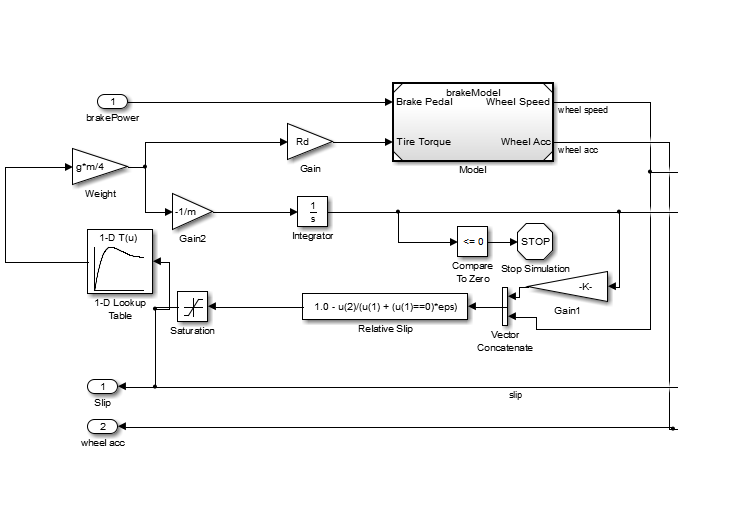
\includegraphics[width=1.0\textwidth]{qrtVehMdl}}

\section{ABS-simulaatioita} \label{app:abssim}
{\centering 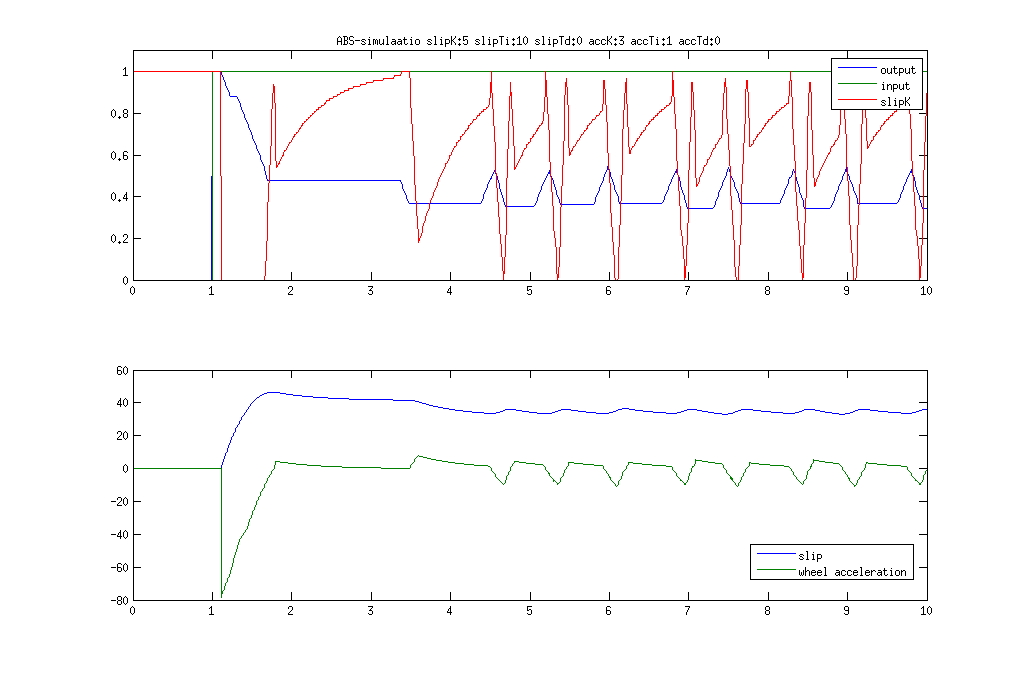
\includegraphics[width=0.8\textwidth]{abssim1}

 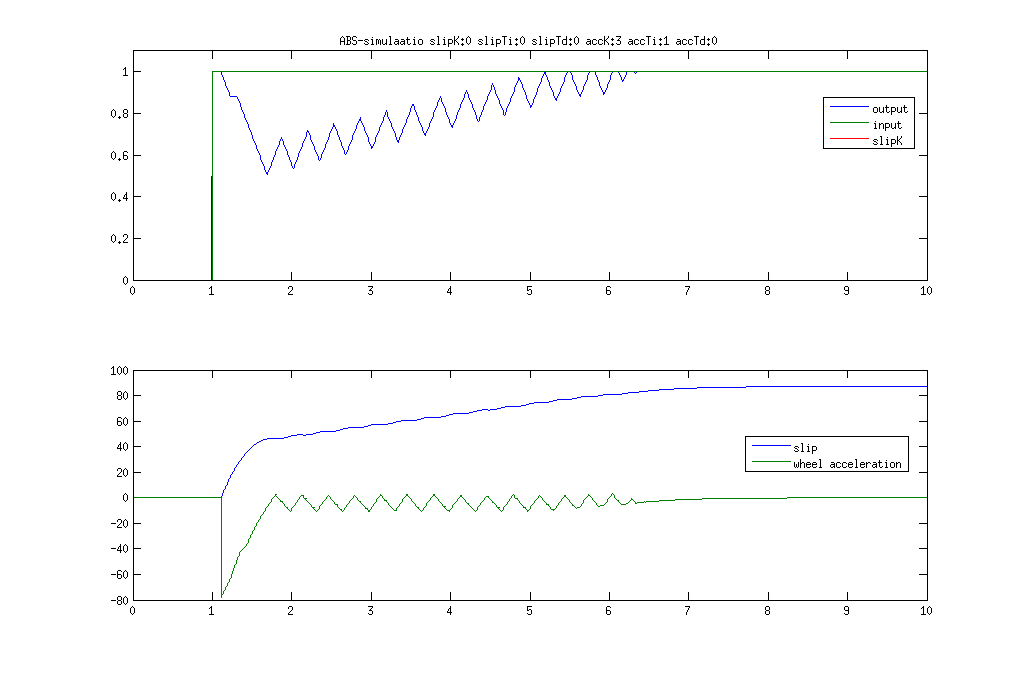
\includegraphics[width=0.8\textwidth]{abssim2}

 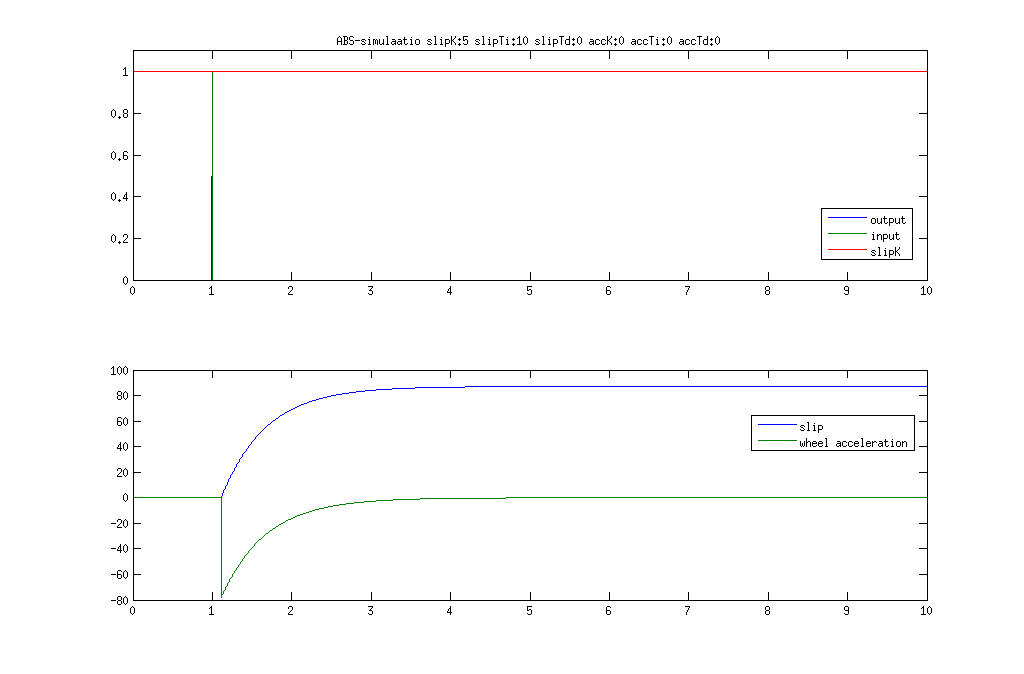
\includegraphics[width=0.8\textwidth]{abssim3}}
%\kuvaa{0.8}{abssim1}{abssim1}{abssim1}
%\kuvaa{0.8}{abssim2}{abssim2}{abssim2}
%\kuvaa{0.8}{abssim3}{abssim3}{abssim3}

\section{ESP-simulaatiomalli} \label{app:espmodel}
{\centering 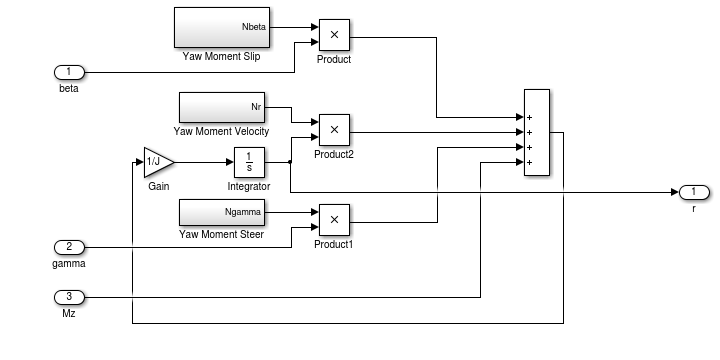
\includegraphics[width=1.0\textwidth]{espmdl1}

 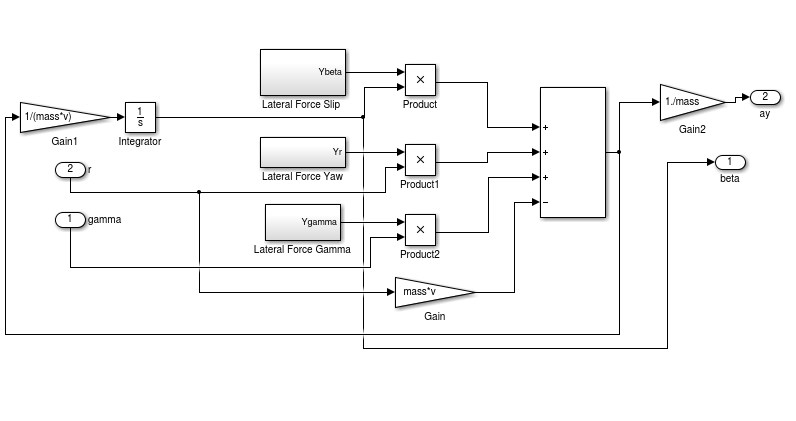
\includegraphics[width=1.0\textwidth]{espmdl2}}
%\kuvaa{0.8}{mdl-a}{mdl-a}{mdl-a}
%\kuvaa{0.8}{mdl-b}{mdl-b}{mdl-b}

\section{ESP-simulaatioita} \label{app:espsim}
{\centering 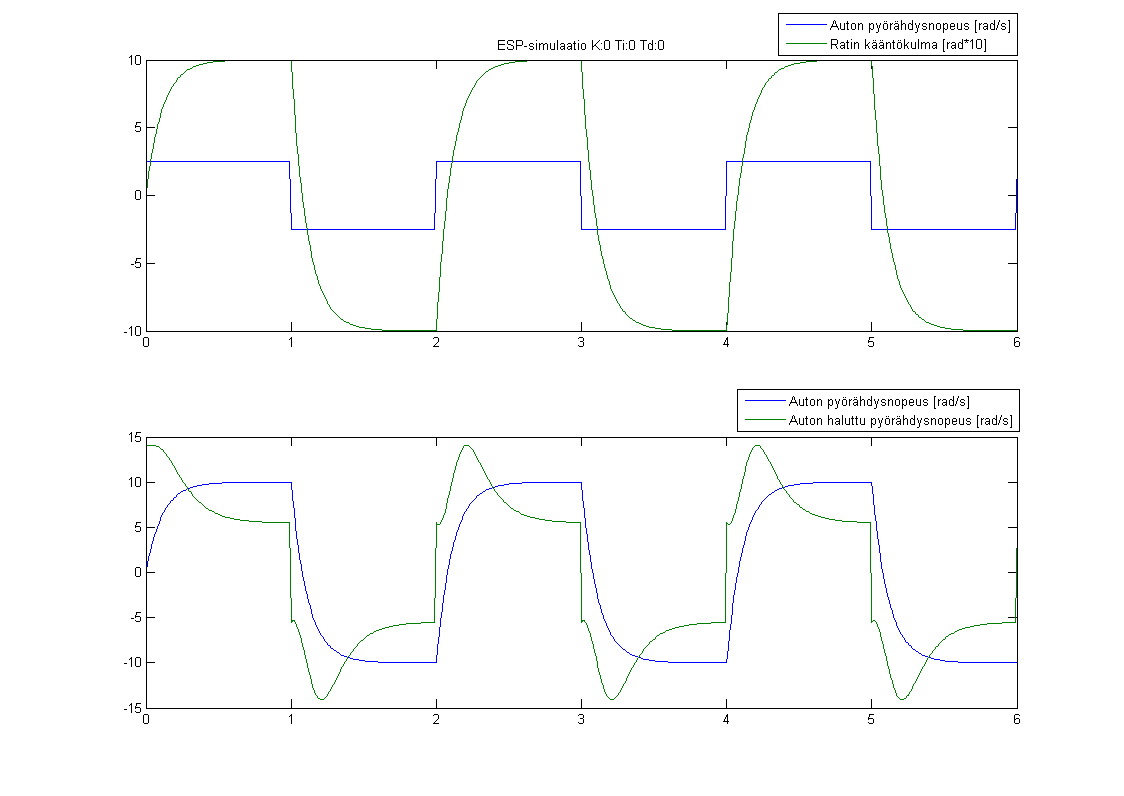
\includegraphics[width=0.8\textwidth]{espSim1}

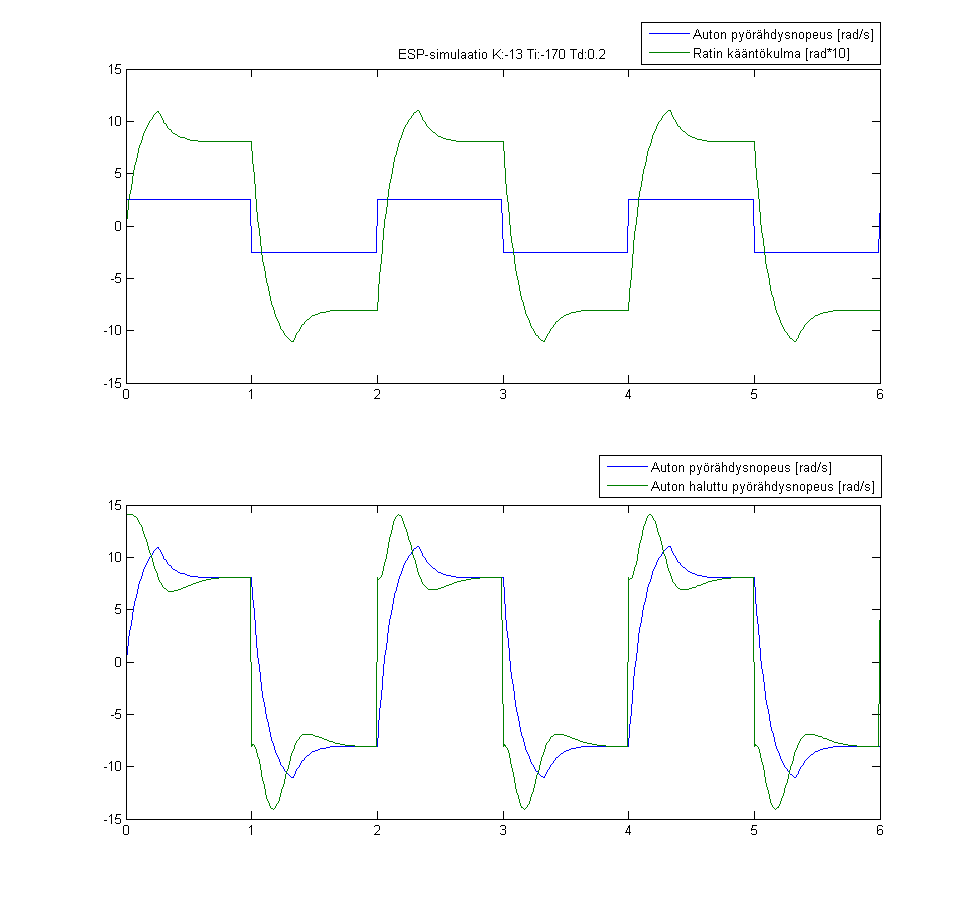
\includegraphics[width=0.8\textwidth]{espSim2}}
\end{appendices}

\end{document}
